\documentclass[a4paper,10pt]{article}
\setlength{\parindent}{0cm}
\usepackage{amsmath, amssymb, amsthm, mathtools,pgfplots}
\usepackage{graphicx,caption}
\usepackage{verbatim}
\usepackage{venndiagram}
\usepackage[cm]{fullpage}
\usepackage{fancyhdr}
\usepackage{tikz}
\usepackage{listings}
\usepackage{color,enumerate,framed}
\usepackage{color,hyperref}
\definecolor{darkblue}{rgb}{0.0,0.0,0.5}
\hypersetup{colorlinks,breaklinks,
            linkcolor=darkblue,urlcolor=darkblue,
            anchorcolor=darkblue,citecolor=darkblue}
\usepackage[utf8]{inputenc}

% Default fixed font does not support bold face
\DeclareFixedFont{\ttb}{T1}{txtt}{bx}{n}{10} % for bold
\DeclareFixedFont{\ttm}{T1}{txtt}{m}{n}{10}  % for normal

% Custom colors
\usepackage{color}
\definecolor{deepblue}{rgb}{0,0,0.5}
\definecolor{deepred}{rgb}{0.6,0,0}
\definecolor{deepgreen}{rgb}{0,0.5,0}

\usepackage{listings}

% Python style for highlighting
\newcommand\pythonstyle{\lstset{
language=Python,
basicstyle=\ttm,
otherkeywords={self},             % Add keywords here
keywordstyle=\ttb\color{deepblue},
emph={MyClass,__init__},          % Custom highlighting
emphstyle=\ttb\color{deepred},    % Custom highlighting style
stringstyle=\color{deepgreen},
frame=tb,                         % Any extra options here
showstringspaces=false            % 
}}


% Python environment
\lstnewenvironment{python}[1][]
{
\pythonstyle
\lstset{#1}
}
{}

% Python for external files
\newcommand\pythonexternal[2][]{{
\pythonstyle
\lstinputlisting[#1]{#2}}}

% Python for inline
\newcommand\pythoninline[1]{{\pythonstyle\lstinline!#1!}}
%\usepackage{tgadventor}
%\usepackage[nohug]{diagrams}
\usepackage[T1]{fontenc}
%\usepackage{helvet}
%\renewcommand{\familydefault}{\sfdefault}
%\usepackage{parskip}
%\usepackage{picins} %for \parpic.
%\newtheorem*{notation}{Notation}
%\newtheorem{example}{Example}[section]
%\newtheorem*{problem}{Problem}
\theoremstyle{definition}
%\newtheorem{theorem}{Theorem}
%\newtheorem*{solution}{Solution}
%\newtheorem*{definition}{Definition}
%\newtheorem{lemma}[theorem]{Lemma}
%\newtheorem{corollary}[theorem]{Corollary}
%\newtheorem{proposition}[theorem]{Proposition}
%\newtheorem*{remark}{Remark}
%\setcounter{section}{1}

\newtheorem{thm}{Theorem}[section]
\newtheorem{lemma}[thm]{Lemma}
\newtheorem{prop}[thm]{Proposition}
\newtheorem{cor}[thm]{Corollary}
\newtheorem{defn}[thm]{Definition}
\newtheorem*{examp}{Example}
\newtheorem{conj}[thm]{Conjecture}
\newtheorem{rmk}[thm]{Remark}
\newtheorem*{nte}{Note}
\newtheorem*{notat}{Notation}

%\diagramstyle[labelstyle=\scriptstyle]

\lstset{frame=tb,
  language=Oz,
  aboveskip=3mm,
  belowskip=3mm,
  showstringspaces=false,
  columns=flexible,
  basicstyle={\small\ttfamily},
  breaklines=true,
  breakatwhitespace=true,
  tabsize=3
}


\pagestyle{fancy}




\fancyhead{}
\renewcommand{\headrulewidth}{0pt}

\lfoot{\color{black!60}{\sffamily Zhangsheng Lai}}
\cfoot{\color{black!60}{\sffamily Last modified: \today}}
\rfoot{\color{black!60}{\sffamily\thepage}}



\begin{document}
\flushright{Zhangsheng Lai\\1002554}
\section*{Statistics: Homework 3}

\begin{enumerate}
\item[10.5] Given $X_1,\ldots,X_n \sim \text{Uniform}(0, \theta)$ and $Y = \max\{X_1,\ldots,X_n\}$, we have the cdf of $Y$ to be $F_Y(y)=(y/\theta)^n$ for $y \in [0,1/2]$.
\begin{enumerate}[(a)]
\item When we choose to reject $H_0$ when $Y>c$, the power function is $\beta(\theta) = 1-(c/\theta)^n$, $c \in [0,1/2]$.
\item Given size of the test to be .05, we need to solve,
\begin{align*}
1-(2c)^n = .05
\end{align*}
which gives us a solution of $c = 1/2(.95)^{1/n}$

\item The size, $\alpha = \beta(1/2) = 1- (2c)^{n}$, $c \in [0,1/2]$. Thus, when $n=20, Y = .48$, the p-value is 
\begin{align*}
\inf\{ \alpha:X^n \in R_\alpha\} = 1-(2 \times.48)^{20} = 0.557997566
\end{align*}
We would conclude that we do not reject $H_0$ with an approximate probability of 0.56, which does not give a strong evidence to reject $H_0$
\item When $n=20, Y = .52$, using the $\alpha$ formula in (c) gives us $1-(2\times.52)^{20} = -1.19112314$. But the given $Y=.52>1/2$ which is out of the defined boundaries of the size, i.e. $F_Y(0.52; \theta=1/2)=0$. Hence the p-value is 0. This allows us to conclude that $H_0$ is to be rejected as the p-value always lies in the critical region; a very strong reason to reject $H_0$.
\end{enumerate}

\item[10.7b] 
Let $H_0: F_T = F_S$ and $H_1: F_T \neq F_S$, where the subscripts denote Twain and Snodgrass respectively. The observed value of the test statistic given by the absolute difference of their means, $|\overline{T} - \overline{S}|$ is 
\begin{align*}
|0.231875 - 0.2097 |=0.022175
\end{align*}
\begin{python}
Have to do some simulation here.
\end{python}
Under this p-value, do we reject $H_0$ at a 5 percent level? How about 2.5 percent level?
\item[10.8]
\begin{enumerate}[(a)]
\item The size of this test with rejection region $R$ is
\begin{align*}
\mathbb{P}(T(X^n)>c| \theta = 0) & = \mathbb{P}(\overline{X}_n > c)\\
& = \mathbb{P}\left(Z > \sqrt{n}c\right), \text{ $Z$ is the standard normal distribution}\\
&= 1- \Phi(\sqrt{n}c), \text{ $\Phi$ is the cdf of the standard normal}
\end{align*}
where by Central Limit Theorem, $\overline{X}_n\sim N(0,1/\sqrt{n})$. Thus given size $\alpha$, the $c$ is $\Phi^{-1}(1-\alpha)/\sqrt{n}$
\item Under $H_1: \theta = 1$, the power is $\beta(1) = \mathbb{P}(T(X^n)>c| \theta = 1) = 1- \Phi\left(\sqrt{n}(c-1)\right)$. 
\item Thus when $n \to \infty$, $\sqrt{n}(c-1)\to \infty$ for $c \neq 1$ which then $1- \Phi\left(\sqrt{n}(c-1)\right) \to 1$.
\end{enumerate}
\item[10.12]
\begin{enumerate}[(a)]
\item We known that the {\sffamily MLE} for $\lambda$ is $\overline{X}_n = n^{-1}\sum_{i=1}^{n}X_i$. The Fisher information $I_n(\lambda)$ is 
\begin{align*}
I_n(\lambda) = nI(\lambda)=-n\mathbb{E}_\lambda\left(\frac{\partial^2 f_X(X;\lambda)}{\partial \lambda^2}\right) = -n\mathbb{E}_\lambda\left(-\frac{X}{\lambda^2}\right)=\frac{n}{\lambda}
\end{align*}
thus by the property of  {\sffamily MLE}, 
\begin{align*}
\frac{\overline{X}_n-\lambda}{\hat{\text{\sffamily se}}} \leadsto N(0,1)
\end{align*}
We reject the null hypothesis if $\left|\frac{\overline{X}_n-\lambda_0}{\sqrt{\lambda_0/n}}\right|>z_{\alpha/2}$ and do not reject otherwise.
%thus the size of of the Wald test
%\begin{align*}
%\mathbb{P}\left(\left|\frac{\overline{X}_n-\lambda_0}{\sqrt{\lambda_0/n}}\right|>z_{\alpha/2}\right)
%\end{align*}
\item 
\begin{python}
import numpy as np
from scipy.stats import norm
def poisson_sample(l, n):
    """
    Generates n Poisson distributed samples with parameter l.
    """
    return np.random.poisson(lam = 1, size = n)
def wald_test(sample, n = 20, alpha = .05, null_lambda = 1):
    """
    Perfoms Wald test and returns p-value.
    """
    xbar = np.mean(sample)
    test_statistic = np.absolute((xbar - null_lambda)/ (null_lambda / n) ** 0.5)
    return  2 * (1 - norm.cdf(test_statistic))
def multwald(l = 1, n = 20, alpha = .05, null_lambda = 1, B = 10000):
    """
    Performs Wald test B times and return proportion of test where null hypothesis is rejected.
    """
    count = 0
    for i in np.arange(B):
        sample = poisson_sample(l, n)
        if wald_test(sample) < alpha:
            count += 1

    return count/B
multwald()            
\end{python}
From performing the simulation of Wald 10000 times, the proportion of null rejected is 0.0564 which is very close to the type I error rate of $\alpha$.
\end{enumerate}
\item[11.3] The posterior density 
\begin{align*}
f(\theta|x^n) &\propto \mathcal{L}_n(\theta)f(\theta)\\
f(\theta|x^n) &\propto (1/\theta)^n(1/\theta)
\end{align*}
Thus the posterior density is a uniform distribution on $(a,b)$ where $b-a=\theta^{n+1}$.


\item[11.4]
\begin{enumerate}
\item The likelihood function where $\theta = (p_1, p_2)$, $X_i \sim \text{Bernoulli}(p_1)$  and $Y_i \sim \text{Bernoulli}(p_2)$ is 
\begin{align*}
\mathcal{L}(\theta)&=p_1^{\sum_{i=1}^{n} X_i}(1-p_1)^{n - \sum_{i=1}^{n} X_i}p_2^{\sum_{i=1}^{n} Y_i}(1-p_2)^{n-\sum_{i=1}^{n} Y_i}\\
\text{with log-likelihood, } \ell(\theta) &=\sum_{i=1}^{n} X_i \log p_1 + \left(n - \sum_{i=1}^{n} X_i\right) \log (1-p_1) +\sum_{i=1}^{n} Y_i \log p_2 + \left(n - \sum_{i=1}^{n} Y_i\right) \log (1-p_2)
\end{align*}
differentiating with respect to $p_1$ and $p_2$ to get the {\sffamily MLE},
\begin{align*}
\frac{\partial \ell}{\partial p_1} &= \frac{\sum_{i=1}^{n} X_i}{p_1} - \frac{\left(n - \sum_{i=1}^{n} X_i\right)}{1-p_1}\\
\frac{\partial \ell}{\partial p_2} &= \frac{\sum_{i=1}^{n} Y_i}{p_2} - \frac{\left(n - \sum_{i=1}^{n} Y_i\right)}{1-p_2}
\end{align*}
we get $\hat{p}_1 = \sum X_i /n$ and $\hat{p}_2 = \sum Y_i /n$ when we solve for the above to be equal to 0. Using the multiparameter delta method, with $\tau = g(\theta) = p_2-p_1$, we have $\hat{\tau} = \hat{p_2} - \hat{p_1}$. We then require $\bigtriangledown \hat{g}$ and $J_n(\hat{\theta})$ to evaluate $\hat{\text{\sffamily se}}(\hat{\tau})$. It is easy to see that $\bigtriangledown \hat{g} = \begin{pmatrix}-1 & 1\end{pmatrix}^T$ and 
\begin{align*}
I_n(\theta) &= \begin{pmatrix} \mathbb{E}_{p_1}\left(\frac{\sum X_i}{p_1^2}+\frac{\left(n - \sum X_i\right)}{(1-p_1)^2}\right) & 0 \\ 0 & \mathbb{E}_{p_1}\left(\frac{\sum Y_i}{p_2^2}+\frac{\left(n - \sum Y_i\right)}{(1-p_2)^2}\right)\end{pmatrix}\\
&= \begin{pmatrix} \frac{n}{p_1}+\frac{n}{(1-p_1)} & 0 \\ 0 & \frac{n}{p_2}+\frac{n}{1-p_2}\end{pmatrix}\\
J_n(\theta) &= \begin{pmatrix} \frac{p_1(1-p_1)}{n} & 0 \\ 0 & \frac{p_2(1-p_2)}{n}\end{pmatrix}
\end{align*}
and thus
\begin{align*}
\hat{\text{\sffamily se}}(\theta)^2=(\bigtriangledown \hat{g})^T J_n(\hat{\theta})(\bigtriangledown \hat{g})=\begin{pmatrix}-1 &1 \end{pmatrix}\begin{pmatrix} \frac{p_1(1-p_1)}{n} & 0 \\ 0 & \frac{p_2(1-p_2)}{n}\end{pmatrix}\begin{pmatrix}-1 \\1\end{pmatrix} = \frac{p_1(1-p_1)}{n} + \frac{p_2(1-p_2)}{n}
\end{align*}
thus $\hat{\text{\sffamily se}}(\hat{\theta}) = \sqrt{\frac{\hat{p}_1(1-\hat{p}_1)}{n} + \frac{\hat{p}_2(1-\hat{p}_2)}{n}}=0.0894427191$ for $n=50$ and the $\hat{p}_1$ and $\hat{p}_2$ obtained earlier. A 90\% confidence interval is $0.2\pm 0.147580487$


\item Using parametric bootstrap, we have {\sffamily MLE} of $p_1$ and $p_2$ to be $\hat{p}_1 = 3/5$ and $\hat{p}_2 = 4/5$ respectively and thus {\sffamily MLE} of $\tau$ to be $1/5$. The parametric bootstrap requires sampling from $X_P \sim \text{Bernoulli}(3/5)$ and $X_T \sim \text{Bernoulli}(4/5)$, where the subscripts denote placebo and treatment respectively. Using 1000 simulations, we get a standard error of 0.0895209919516.
\begin{python}
import numpy as np

mle_p1 = 3/5
mle_p2 = 4/5
mle_tau = mle_p2 - mle_p1
n = 100000

se2_boot = 0

for i in np.arange(n):
    p1_mean = np.mean(np.random.binomial(1, mle_p1, size = 50))
    p2_mean = np.mean(np.random.binomial(1, mle_p2, size = 50))
    se2_boot += ((p2_mean - p1_mean) - mle_tau) ** 2
se_boot = np.sqrt(se2_boot/n)
print (se_boot)
\end{python}
A 90\% confidence interval will then be $0.2 \pm 0.148$



\item With the prior $f(p_1,p_2) = 1$, 
\begin{align*}
f(p_1,p_2|x^n,y^n) \propto \mathcal{L}(p_1,p_2)= p_1^{\sum_{i=1}^{n} X_i}(1-p_1)^{n-\sum_{i=1}^{n} X_i}p_2^{\sum_{i=1}^{n} Y_i}(1-p_2)^{n-\sum_{i=1}^{n} Y_i}
\end{align*}
and since
\begin{align*}
f(p_1,p_2|x^n,y^n) &= f(p_1|x^n)f(p_2|y^n)\\
\text{ and }f(p_1|x^n)&\propto p_1^{\sum_{i=1}^{n} X_i}(1-p_1)^{n-\sum_{i=1}^{n} X_i}\\
f(p_2|y^n)&\propto p_2^{\sum_{i=1}^{n} Y_i}(1-p_2)^{n-\sum_{i=1}^{n} Y_i}
\end{align*}
the simulation is by drawing samples from $p_1 | x^n \sim \text{Beta}(31,21)$ and $p_2 | y^n \sim \text{Beta}(41,11)$ which gives a posterior mean estimate of $\tau$ to be 0.19313 with the code below:
\begin{python}
n = 1000

p1 = np.random.beta(31, 21, size = n)
p2 = np.random.beta(41, 11, size = n)

np.mean(p2 - p1)
\end{python}
we then plot a histogram 
\begin{figure}[h]
\centering
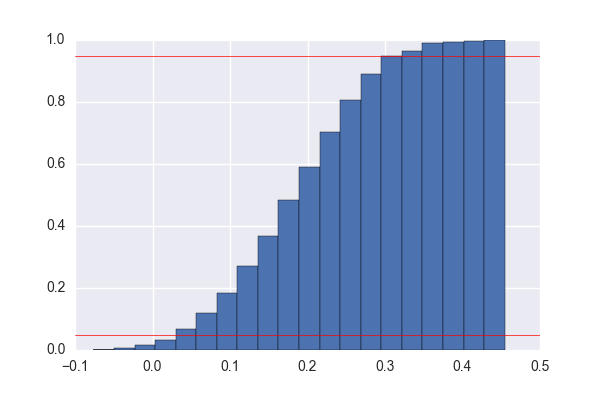
\includegraphics[scale=1]{posteriorCI1.png}
\caption{Cumulative distribution to obtain posterior confidence interval}
\end{figure}
with the code below
\begin{python}
n = 1000

p1 = np.random.beta(31, 21, size = n)
p2 = np.random.beta(41, 11, size = n)

tau = p2 - p1

plt.hist(tau, cumulative = True, normed = True, bins = 20)
plt.axhline(y = 0.05, color = 'r', linewidth = 0.5)
plt.axhline(y = 0.95, color = 'r', linewidth = 0.5)
\end{python}
and see that a 90\% confidence interval by simulation is approximately $(0.023248,0.36918)$.


\item The {\sffamily MLE} of $\psi$ is $\log\left(\frac{3/5}{2/5}\div\frac{4/5}{1/5}\right) = \log 3/8$. Using the multiparameter delta method, $\bigtriangledown g = \begin{pmatrix}\frac{1}{p_1(1-p_1)}&-\frac{1}{p_2(1-p_2)}\end{pmatrix}$ and with $J_n(\theta)$ from earlier
\begin{align*}
\hat{\text{\sffamily se}}(\theta)^2 = (\bigtriangledown \hat{g})^T J_n(\hat{\theta}) (\bigtriangledown \hat{g}) &= \begin{pmatrix}\frac{1}{p_1(1-p_1)}&-\frac{1}{p_2(1-p_2)}\end{pmatrix}\begin{pmatrix} \frac{p_1(1-p_1)}{n} & 0 \\ 0 & \frac{p_2(1-p_2)}{n}\end{pmatrix}\begin{pmatrix}\frac{1}{p_1(1-p_1)}\\-\frac{1}{p_2(1-p_2)}\end{pmatrix}\\
&=\frac{1}{np_1(1-p_1)}+\frac{1}{np_2(1-p_2)}
\end{align*}
thus $\hat{\text{\sffamily se}}(\hat{\theta}) = \sqrt{\frac{1}{n\hat{p}_1(1-\hat{p}_1)}+\frac{1}{n\hat{p}_2(1-\hat{p}_2)}} = 0.456435465$. A 90\% confidence interval would be $\log3/8 \pm 0.753118517$


\item The posterior estimate of $\psi$ is 0.94397 and the posterior 90\% interval for $\psi$ is $(-1.68,-0.416)$

\begin{python}
n = 1000

p1 = np.random.beta(31, 21, size = n)
p2 = np.random.beta(41, 11, size = n)

psi_distribution = np.log((p1 / (1 - p1)) / (p2 / (1 - p2)))

psi_estimate = np.mean(psi_distribution)

print (psi_estimate)

plt.axhline(y = 0.05, color = 'r', linewidth = 0.5)
plt.axhline(y = 0.95, color = 'r', linewidth = 0.5)

plt.hist(psi_distribution, cumulative = True, normed = True, bins = 20)

\end{python}

\begin{figure}[h]
\centering
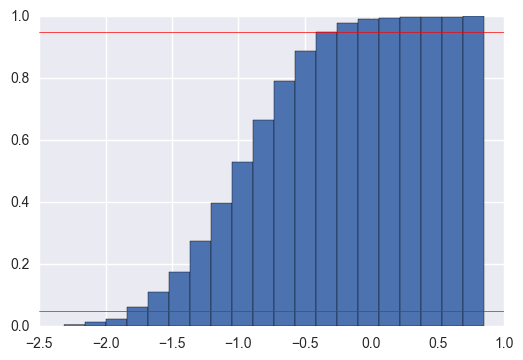
\includegraphics[scale=1]{psiposteriorCI1.png}
\caption{Cumulative distribution to obtain $ \psi$ posterior confidence interval}
\end{figure}


\end{enumerate}
\end{enumerate}

\end{document}